\begin{frame}
	\begin{columns}
		\begin{column}{0.5\textwidth}
			\textit{``\dots not because they are easy,
				but because they are hard\dots''}
			~ \\ ~ \\
			\footnotesize
			\hfill{} -- John F. Kennedy \\
			\hfill{}	12. Spetember, 1962
		\end{column}
		\begin{column}{0.5\textwidth}
			\begin{figure}
				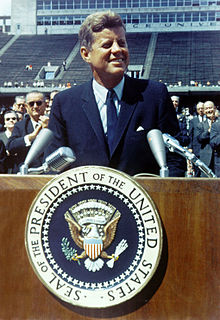
\includegraphics[scale=2]{../../fig/kennedy_01.jpg}
				\caption{\footnotesize
					John F. Kennedy bei seiner Mond-Rede an
					der Rice Universität (Quelle: Wikipedia)}
			\end{figure}
		\end{column}
	\end{columns}
\end{frame}
